\documentclass[a4paper]{article}

\usepackage[utf8]{inputenc}
\usepackage[T1]{fontenc}
\usepackage[frenchb]{babel}
\usepackage{colortbl}
\usepackage{graphicx}
\usepackage{moresize}
\usepackage{anyfontsize}
\usepackage{hyperref}
\usepackage{longtable}
\usepackage[table]{xcolor}
\usepackage{tabularx}
\usepackage{pdfpages}
\usepackage{pdflscape}
\usepackage{lastpage}
\usepackage{array}
 \usepackage{float}
\usepackage{caption}
\usepackage{wrapfig}

% Definition des pages
\usepackage[left=3cm,right=3cm,top=3cm,bottom=3cm]{geometry}

% En-tete de page
\usepackage{fancyhdr}
\pagestyle{fancy}

% Lien hypertexte
\usepackage{hyperref}
\hypersetup{
  hidelinks,
  backref=true,
  pagebackref=true,
  hyperindex=true,
  colorlinks=false,
  breaklinks=true,
  urlcolor=ocre,
  bookmarks=true,
  bookmarksopen=false,
  pdftitle={Compte Rendu JEE},
  pdfauthor={Yohann HENRY - Jérémie PANTIN}
}

\definecolor{purp}{RGB}{110, 40, 150}
\definecolor{grisC}{RGB}{245, 245, 245}
\definecolor{grisF}{RGB}{224, 224, 224}
\definecolor{grisP}{RGB}{136, 136, 136}
\definecolor{ocre}{RGB}{51,102,0}

\makeatletter
\renewcommand{\@seccntformat}[1]{\llap{\textcolor{purp}{\csname the#1\endcsname}\hspace{1em}}}                    
\renewcommand{\section}{\@startsection{section}{1}{\z@}
{-4ex \@plus -1ex \@minus -.4ex}
{1ex \@plus.2ex }
{\normalfont\large\sffamily\bfseries}}
\renewcommand{\subsection}{\@startsection {subsection}{2}{\z@}
{-3ex \@plus -0.1ex \@minus -.4ex}
{0.5ex \@plus.2ex }
{\normalfont\sffamily\bfseries}}
\renewcommand{\subsubsection}{\@startsection {subsubsection}{3}{\z@}
{-2ex \@plus -0.1ex \@minus -.2ex}
{.2ex \@plus.2ex }
{\normalfont\small\sffamily\bfseries}}                        
\renewcommand\paragraph{\@startsection{paragraph}{4}{\z@}
{-2ex \@plus-.2ex \@minus .2ex}
{.1ex}
{\normalfont\small\sffamily\bfseries}}

\renewcommand\headrulewidth{1pt}
\fancyhead[L]{
\includegraphics[height=1cm]{resources/univ.png}}
\fancyhead[C]{Compte Rendu\\ \color{grisP}\texttt{Projet JEE}}
\fancyfoot[C]{\texttt{\thepage/\pageref{LastPage}}}
\makeatletter
\newcommand{\resetHeadWidth}{\fancy@setoffs}
\makeatother


\renewcommand{\arraystretch}{1.5}

\begin{document}

\begin{titlepage}
	\begin{center}
		{\fontsize{22}{30}\selectfont Projet Architectures Orientées Services sous JEE\\Guide d'utilisation}\\[\baselineskip]
		\vspace*{10pt}
		{\Large\itshape 19/01/2017}\\
		\vfill
		\rule{0.6\textwidth}{0.4pt}\\[\baselineskip]
		\begin{table}[h]
			\centering
			\def\arraystretch{1.4}
			\begin{tabular}{ll|ll}
				Yohann & HENRY & Jérémie & PANTIN\\
			\end{tabular}
		\end{table}
	\end{center}
\end{titlepage}

\thispagestyle{empty}

\tableofcontents
\newpage
\setcounter{page}{1}
\vspace*{0.5cm}

\section{Introduction}
Ce document a pour but d'indiquer comment installer l'application web afin de la faire marcher sur sa propre machine. Il y a toutefois des pré-requis à avoir afin de pouvoir exécuter les commandes.

\section{Pré-requis}
\subsection{Système d'exploitation}
L'application a été développée sur deux OS :
\begin{itemize}
\item Windows (10)
\item Ubuntu
\end{itemize}

Ainsi nous n'assurons aucunement la bon déroulement sur d'autres systèmes d'exploitation.

\subsection{Base de données}
Il est nécessaire également de posséder une base de données afin d'assurer la persistance de l'application. Plus précisément : \texttt{PostgreSQL}. En effet l'application est prévue pour fonctionner sur une SGBD PostgreSQL.\\
Nous prévoyons deux cas lors du déploiement de l'application, une en prenant les configurations définies dans les sources (sans modifications). Un autre cas consiste à modifier le fichier de configuration afin d'appliquer par rapport à votre propre contexte.

\subsubsection{Cas 1}
La configuration demandée par l'application, telle quelle , est la suivante :
\begin{itemize}
\item User : postgres
\item Password : postgres
\item Une base : jeedb
\end{itemize}

\subsubsection{Cas 2}
Modification dans le fichier \texttt{\textbf{NotifCosmoEI/src/main/resources/application.properties}}

\begin{figure}[h]
\centering
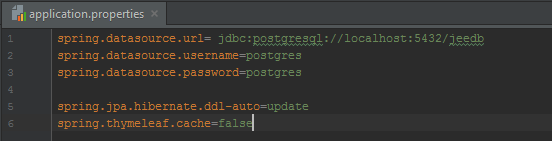
\includegraphics[scale=1]{resources/cas_2.png}
\caption{Fichier de propriété}
\end{figure}

\subsection{Maven}
Vérifier que \texttt{Maven} est présent sur la machine et dans les environnements de variables.

\newpage

\section{Lancement de l'application}
Pour lancer l'application et la construire (les deux se font en même temps), il faut lancer la commande suivant :\\
\texttt{mvn clean spring-boot:run}

\begin{figure}[h]
\centering
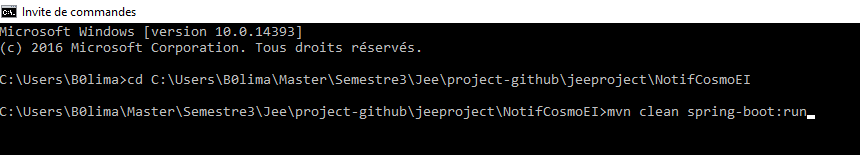
\includegraphics[scale=.7]{resources/start1.png}
\caption{Lancement}
\end{figure}

\begin{figure}[h]
\centering
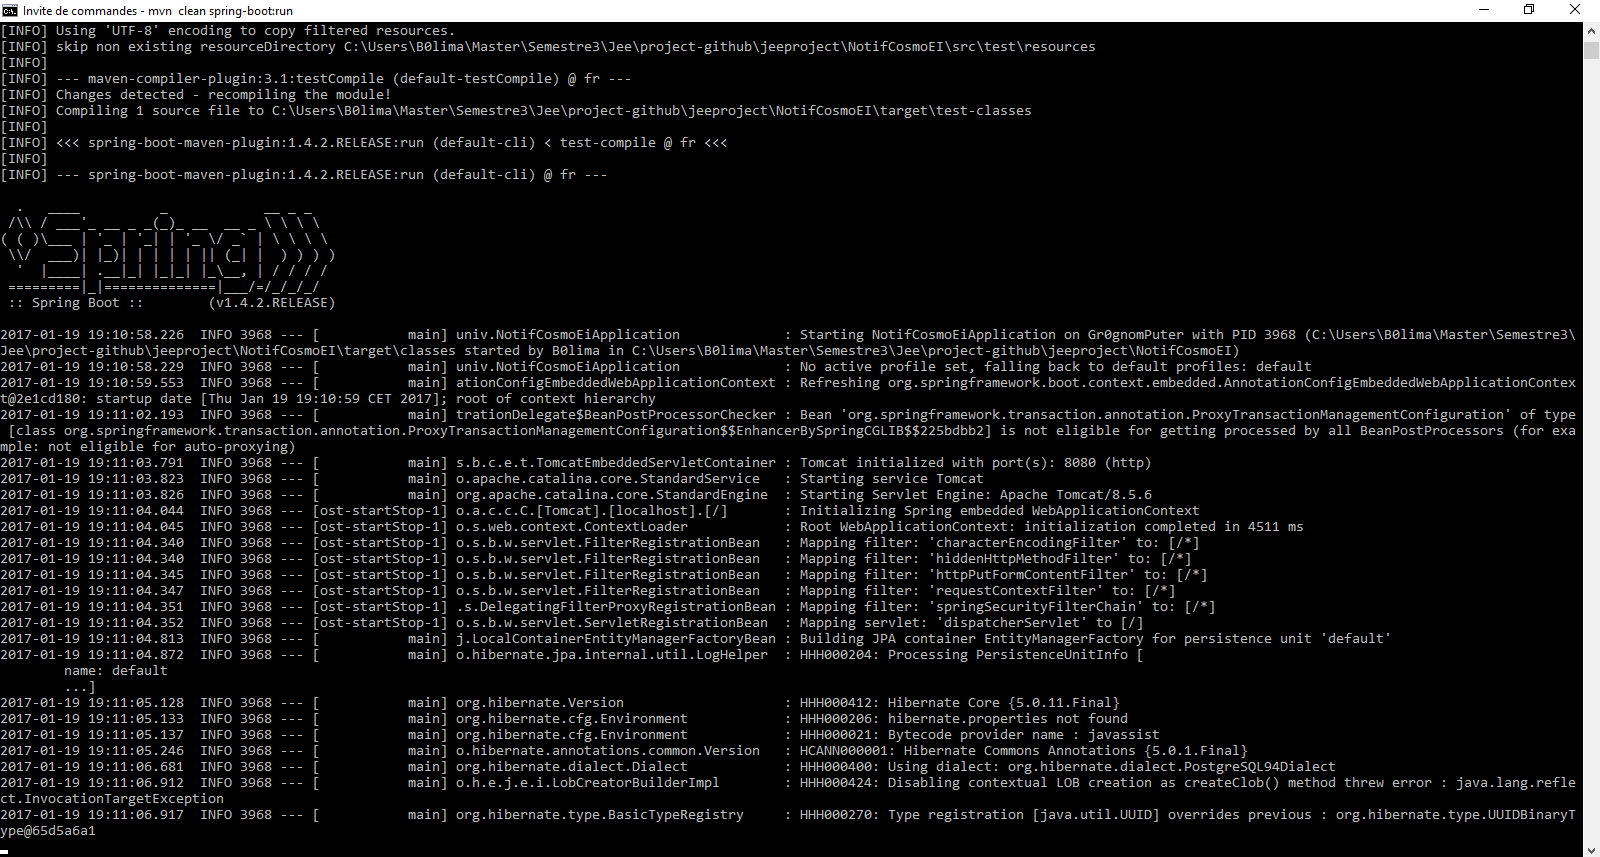
\includegraphics[scale=.3]{resources/start2.png}
\caption{Build}
\end{figure}

\begin{figure}[h]
\centering
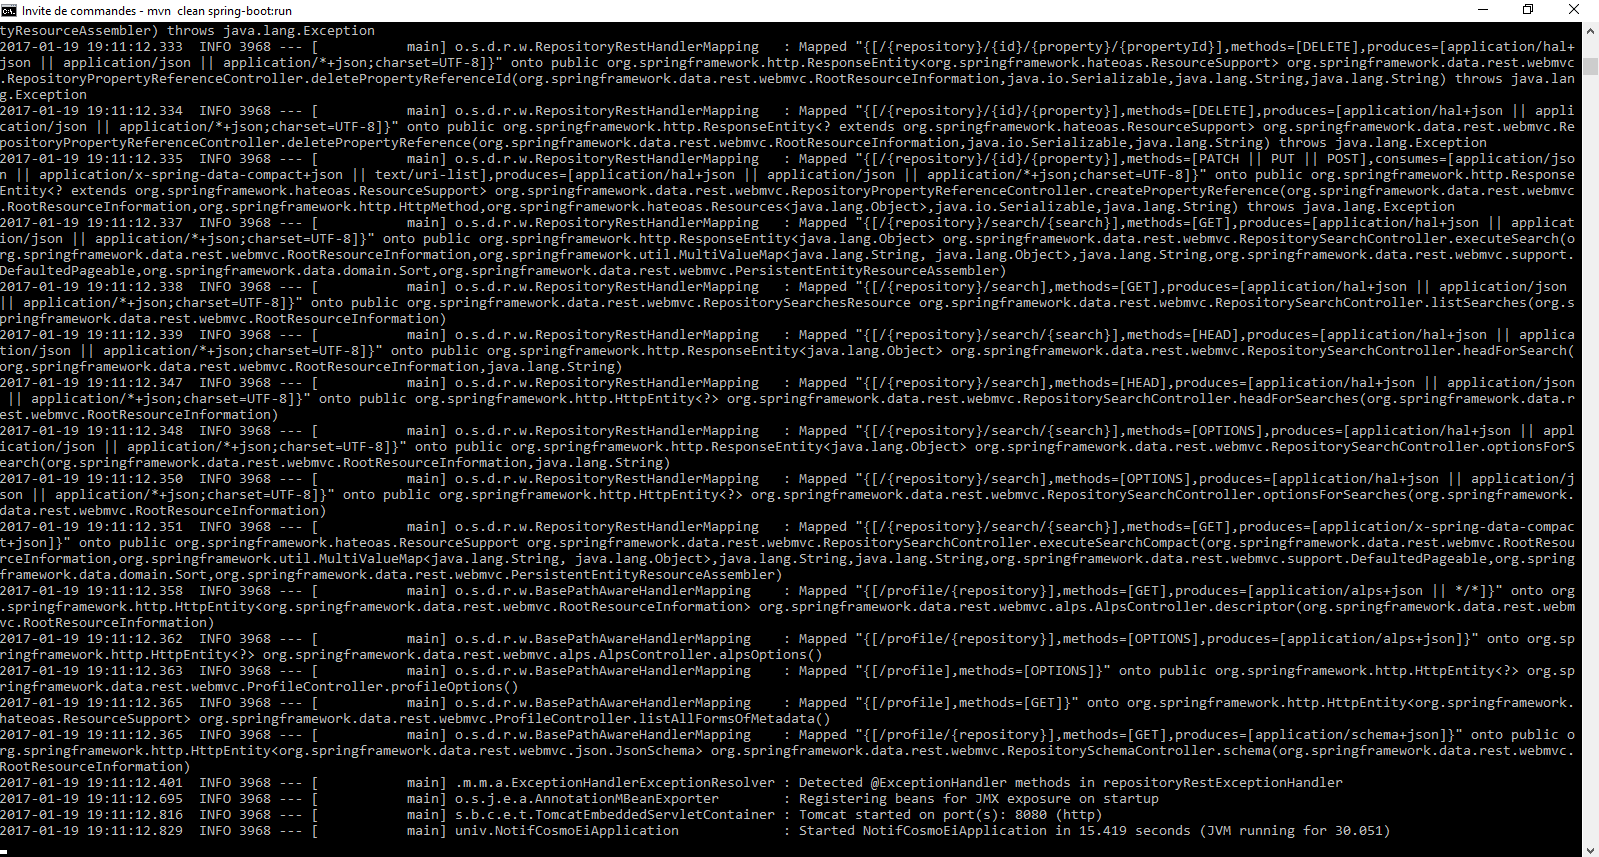
\includegraphics[scale=.2]{resources/start3.png}
\caption{Application prête à l'emploi}
\end{figure}

\section{Utiliser}
Il ne reste plus qu'à aller sur un navigateur Web et aller sur l'URL : \texttt{localhost:8080}

\end{document}